\documentclass[12pt,a4paper]{article}

\usepackage[margin=2.5cm]{geometry}
\usepackage{amsmath}
\usepackage{graphicx}
\usepackage{float}
\usepackage[hidelinks]{hyperref}

\usepackage{polyglossia}
\setmainlanguage[numerals=arabic]{armenian}
\setmainfont{FreeSerif}
\newfontfamily\armenianfonttt{FreeSerif}

\sloppy

\title{Չերենկովյան ճառագայթում}
\date{}

\begin{document}
\maketitle

Ըստ Էյնշտեյնի հանրահայտ հարաբերականության տեսության՝ ոչ մի մասնիկի
արագությունը չի կարող գերազանցել լույսի արագությունը, սակայն գիտության
մեջ դիտվել են դեպքեր, երբ մասնիկների արագությունները գերազանցել են
լույսի արագությունը\ldots{} (խոսքը, իհարկե, միջավայրում լույսի արագության
մասին է :D)

Պատճառն այն է, որ այդ մասնիկները գերազանցել են լույսի փուլային
արագությունն իրենց միջավայրում, իսկ ըստ Էյնշտեյնի՝ լույսի արագությունն
անգերազանցելի է վակուումում: Առաջին անգամ այդ երևույթին ականատես է եղել
ռուս գիտնական Չերենկովը՝ նկատելով ջրի մեջ կապույտ գույնի ճառագայթում
(նկ.~\ref{fig:glow}), երբ այն գտնվում էր գամմա ճառագայթման ազդեցության տակ: Ի
սկզբանե նա մտածում էր, որ այդ երևույթի պատճառը
լյումինեսցենցումն\footnote{\url{https://ru.wikipedia.org/wiki/Люминесценция}} է՝
տվյալ ջերմաստիճանում մարմնի ջերմային ճառագայթման նկատմամբ ավելցուկային
լուսարձակումը, որը նույնպես ուղեկցվում է կապույտ գույնի ճառագայթմամբ:
Սակայն ի տարբերություն լյումինեսցենցման, Չերենկովի դիտարկած դեպքում
ճառագայթումը դիտվում էր բոլոր թափանցիկ հեղուկների դեպքում: Ավելին՝
ճառագայթումը շատ քիչ էր կախված նյութի քիմիական բաղադրությունից: Այս
տարբերությունների հիման վրա Չերենկովն ու Վավիլովը եզրակացրեցին, որ
դիտարկված երևույթի պատճառն իրականում ոչ թե լյումինեսցենցումն է, այլ այդ
լույսը ճառագայթում են հեղուկի մեջ շարժվող էլեկտրոնները: Իսկ այդ
էլեկտրոնները առաջանում են Քոմփթոնի էֆեկտի պատճառով, ըստ որի գամմա
ճառագայթումը էլեկտրոն է պոկում մասնիկի էլեկտրոնային թաղանթից, նրան մեծ
իմպուլս հաղորդելով, որի արդյունքում էլ էլեկտրոնը շարժվում է միջավայրում
լույսի արագությունից մեծ արագությամբ ու ճառագայթում կապույտ գույնի
լույս:

\begin{figure}[H]
  \centering
  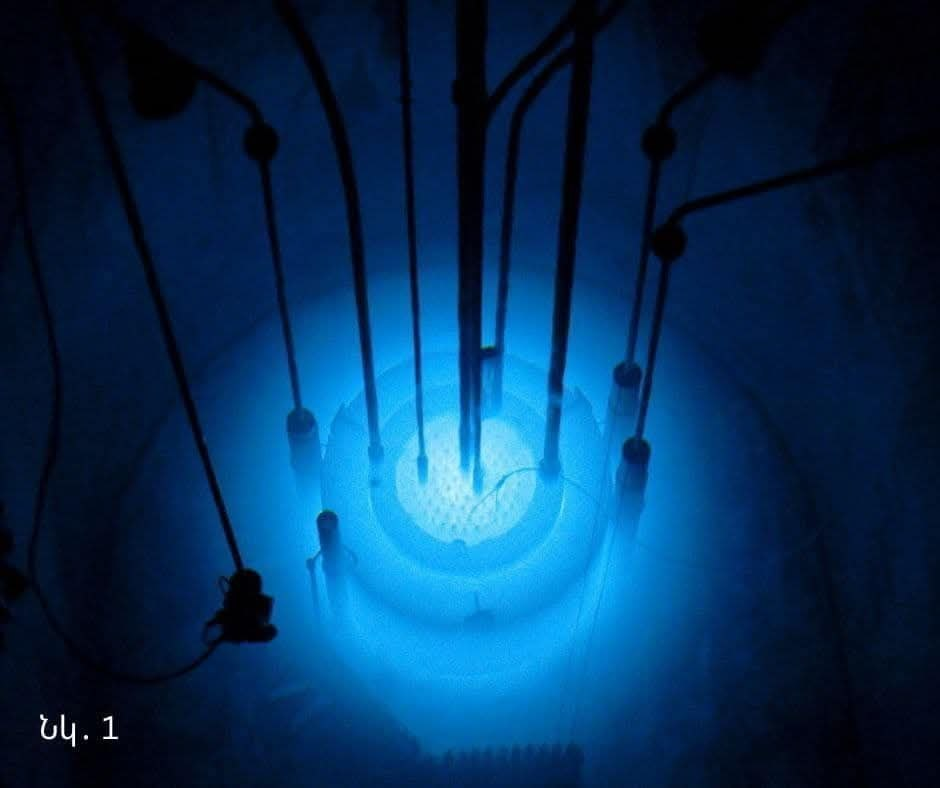
\includegraphics[width=0.55\textwidth]{images/img1.png}
  \caption{Չերենկովյան ճառագայթում ջրի մեջ:}
  \label{fig:glow}
\end{figure}

Ըստ քվանտային տեսության՝ լույսն իրենից ներկայացնում է լույսի քվանտների՝
ֆոտոնների հոսք: Դրանցից ամեն մեկն ունի իրեն համապատասխան էներգիան՝
\begin{equation}
  E = h\nu = \frac{hc}{\lambda},
\end{equation}
և իմպուլսը՝
\begin{equation}
  p = \frac{h}{\lambda}.
\end{equation}
Այստեղ $\nu$-ն ֆոտոնի հաճախությունն է, $\lambda$-ն՝ ալիքի երկարությունը, իսկ
$h$-ը՝ Պլանկի հաստատունը:

Ըստ Քոմփթոնի\footnote{\url{https://hy.wikipedia.org/wiki/Քոմփթոնի_էֆեկտ}}՝
էլեկտրոնից ցրվելիս էլեկտրամագնիսական ալիքի երկարությունը մեծանում է:
Սկզբում ֆոտոնի էներգիան $h\nu$ է, և այն ունի այդ էներգիային համապատասխան
$\lambda$ ալիքի երկարություն: Էլեկտրոնի հետ բախումից հետո ֆոտոնն իր էներգիայի և
իմպուլսի մի մասը տալիս է էլեկտրոնին: Ֆոտոնի էներգիան փոքրանում է, և այն
շարժվում է սկզբնական ուղղության նկատմամբ $\theta$ անկյան տակ՝ արդեն ավելի փոքր
$h\nu'$ էներգիայով, որին համապատասխանում է սկզբնականից ավելի մեծ $\lambda'$
ալիքի երկարություն (նկ.~\ref{fig:compton}):

\begin{figure}[H]
  \centering
  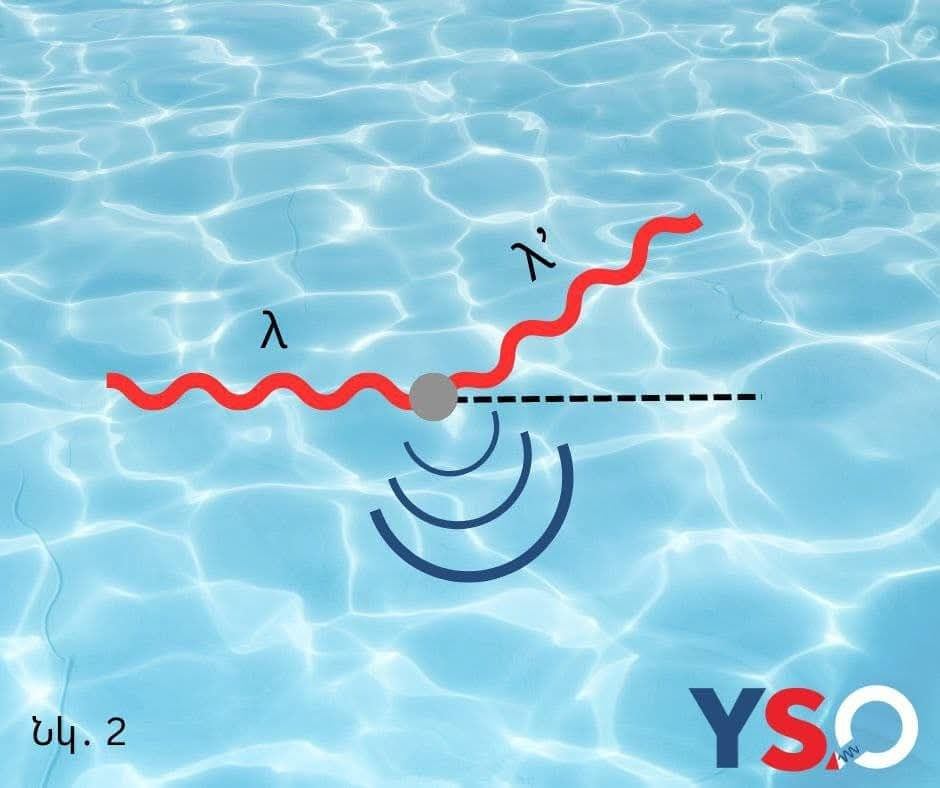
\includegraphics[width=0.6\textwidth]{images/img2.png}
  \caption{Քոմփթոնի ցրում:}
  \label{fig:compton}
\end{figure}

Վավիլով--Չերենկովի էֆեկտը բացատրվում է Հյուգենս--Ֆրենելի սկզբունքով: Այն
ձևակերպելուց առաջ ծանոթանանք գերձայնային ինքնաթիռների աշխատանքի
սկզբունքին:

Սովորական ինքնաթիռի թռիչքի ժամանակ ինքնաթիռը շարժում է օդը, որի միջով
շարժվում է (նկ.~\ref{fig:subsonic}): Այդ շարժումը բերում է ինքնաթիռի շուրջ օդի հոսքին և
ճնշումային ալիքի առաջացմանը, որը մենք ձայնի տեսքով ենք ընկալում:
Գերձայնային ինքնաթիռի թռիչքի ժամանակ օդի խանգարումներն ընկնում են
ինքնաթիռից հետ, քանի որ այն ձայնից արագ է շարժվում (նկ.~\ref{fig:sonic}, \ref{fig:supersonic}): Իսկ
ճնշումային ալիքի առաջացման փոխարեն դրանք միավորվում են ու ստեղծում
հարվածային ալիք, որը մարդիկ ընկալում են որպես ձայնային պայթյուն: Դրան
շատ նման սկզբունքով է աշխատում Հյուգենսի սկզբունքը օպտիկայում:

\begin{figure}[H]
  \centering
  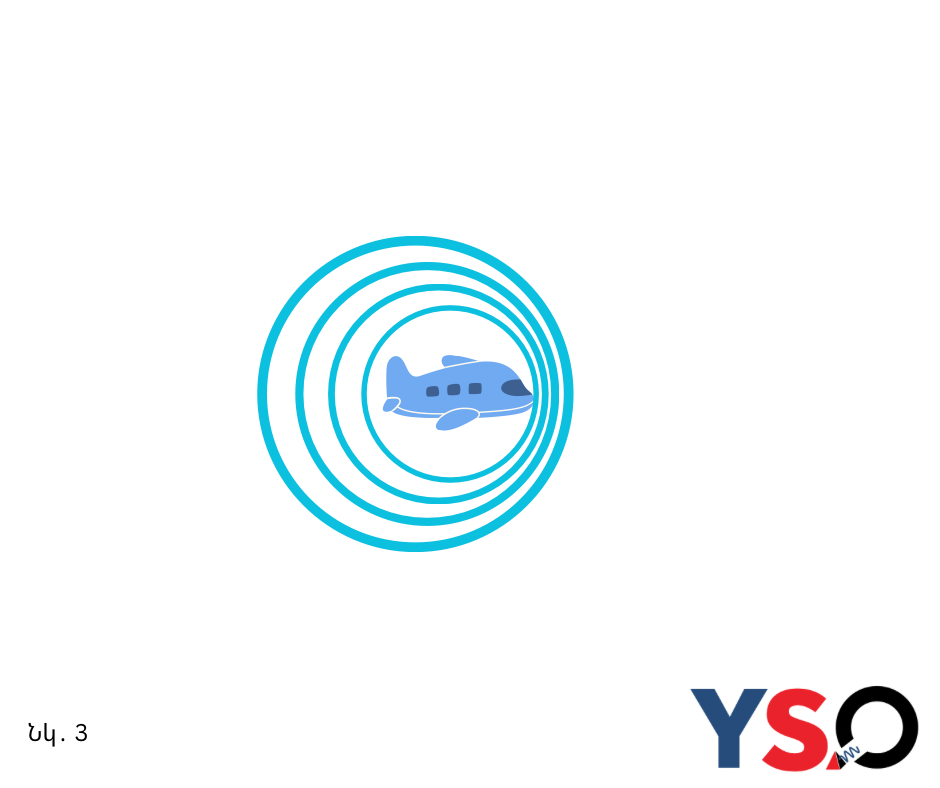
\includegraphics[width=0.6\textwidth]{images/img3.png}
  \caption{Սովորական (ենթաձայնային) ինքնաթիռ:}
  \label{fig:subsonic}
\end{figure}

\begin{figure}[H]
  \centering
  \begin{minipage}{0.48\textwidth}
    \centering
    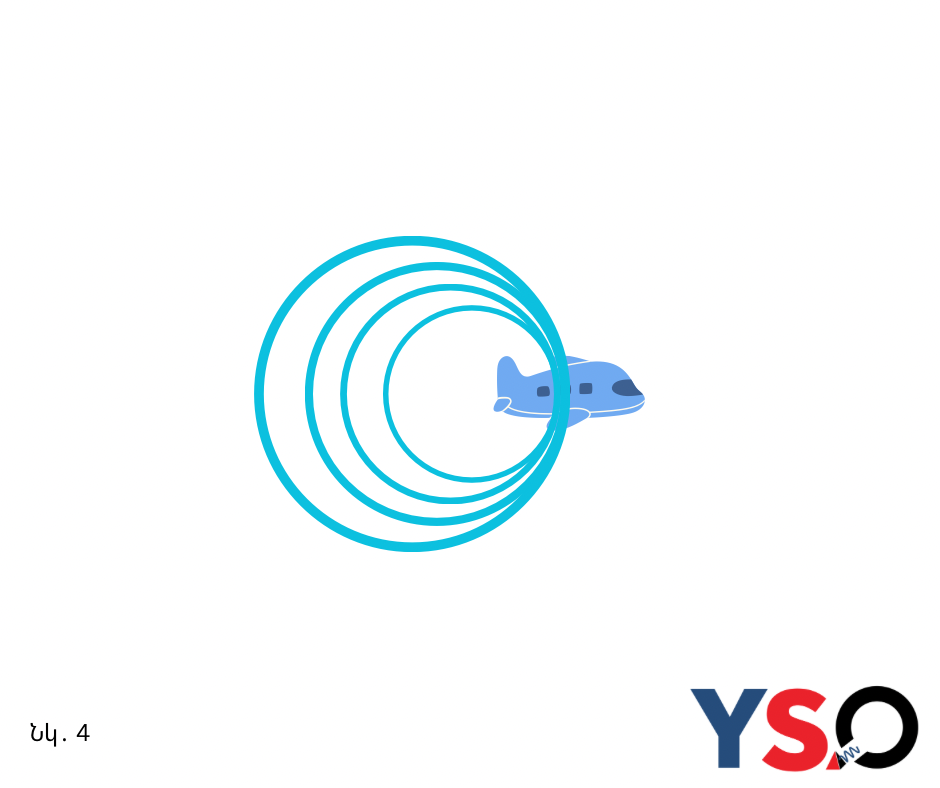
\includegraphics[width=\linewidth]{images/img4.png}
    \caption{Գերձայնային ինքնաթիռ:}
    \label{fig:sonic}
  \end{minipage}
  \hfill
  \begin{minipage}{0.48\textwidth}
    \centering
    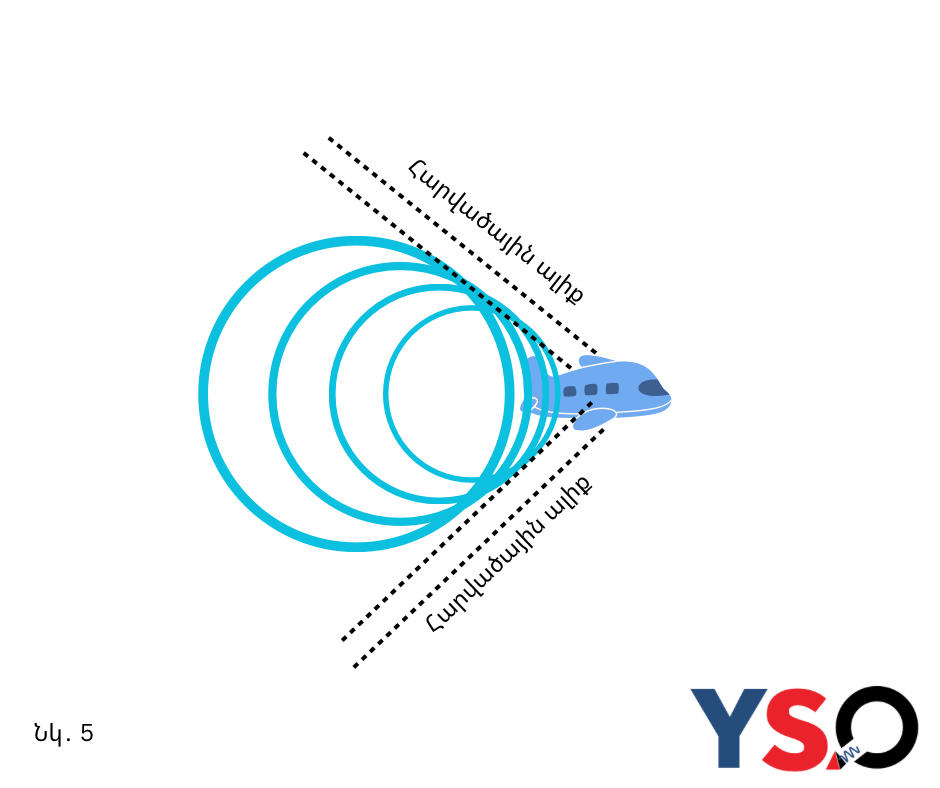
\includegraphics[width=\linewidth]{images/img5.png}
    \caption{Հարվածային ալիք:}
    \label{fig:supersonic}
  \end{minipage}
\end{figure}

Հյուգենսը պնդում էր, որ մակերևույթի յուրաքանչյուր կետ, որին հասել է
լուսային ալիքը, ալիքների երկրորդային աղբյուր է: Այս սկզբունքի շնորհիվ
ամբողջ ալիքային պրոցեսի փոխարեն կարող ենք դիտարկել կամայականորեն ընտրված
ալիքային մակերևույթ: Այսինքն՝ եթե լիցքավորված մասնիկն անցել է նկարում
պատկերված $A, B, C, D, E$ կետերով (նկ.~\ref{fig:points}), դրանք կարող ենք համարել ալիքի
առաջացման աղբյուր հենց այն պահին, երբ մասնիկն անցնում է այդ
կետերով:

\begin{figure}[H]
  \centering
  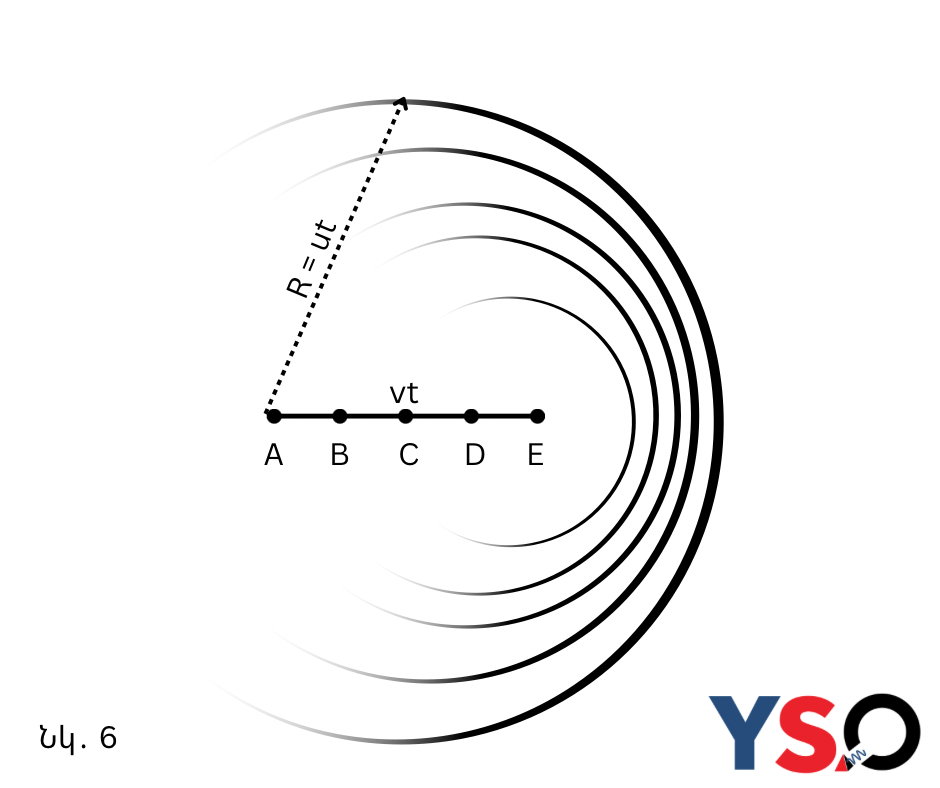
\includegraphics[width=0.6\textwidth]{images/img6.png}
  \caption{Մասնիկի հետագիծը և $A, B, C, D, E$ կետերը ($v<u$):}
  \label{fig:points}
\end{figure}

Հիմա ենթադրենք, որ մասնիկը շարժվում է $v$ արագությամբ ու մեր դիտարկած
պահին այն $E$ կետում է գտնվում: $t$ ժամանակ առաջ այն գտնվում էր $A$ կետում, և
այդ կետերի միջև հեռավորությունը $vt$ է: Այսինքն $A$ կետում առաջացած ալիքը
մեր դիտարկած պահին իրենից կներկայացնի $ut$ շառավղով շրջանագիծ, որտեղ $u$-ն
լույսի արագությունն է միջավայրում և
\begin{equation}
  u = \frac{c}{n}
\end{equation}
($n$-ը միջավայրի բեկման ցուցիչն է): Այսպես $B$, $C$, $D$ կետերում գնալով ավելի ուշ է ալիք
ճառագայթվել:

Ստացվում է, որ եթե մասնիկի արագությունը լույսի փուլային արագությունից
փոքր է, լույսը կվազանցի մասնիկը: Եվ ինչքան շուտ է ճառագայթվել լուսային
ալիքը, այդքան անգամ շատ լույսը մասնիկից առաջ կընկնի, ու արդյունքում
մասնիկից լույս չի ճառագայթվի:

Սակայն երբ մասնիկի արագությունը մեծ է լույսի փուլային արագությունից,
պատկերն այլ տեսք է ստանում (նկ.~\ref{fig:cone}).

Լույսի ալիքի ճակատներն արդեն հատվում են, և այդ հատման կետերի ընդհանուր
շոշափողները հատվում են մեր դիտարկած $E$ կետում: Իսկ սլաքներով նշված են
լույսի ճառագայթման ուղղությունները:

\begin{figure}[H]
  \centering
  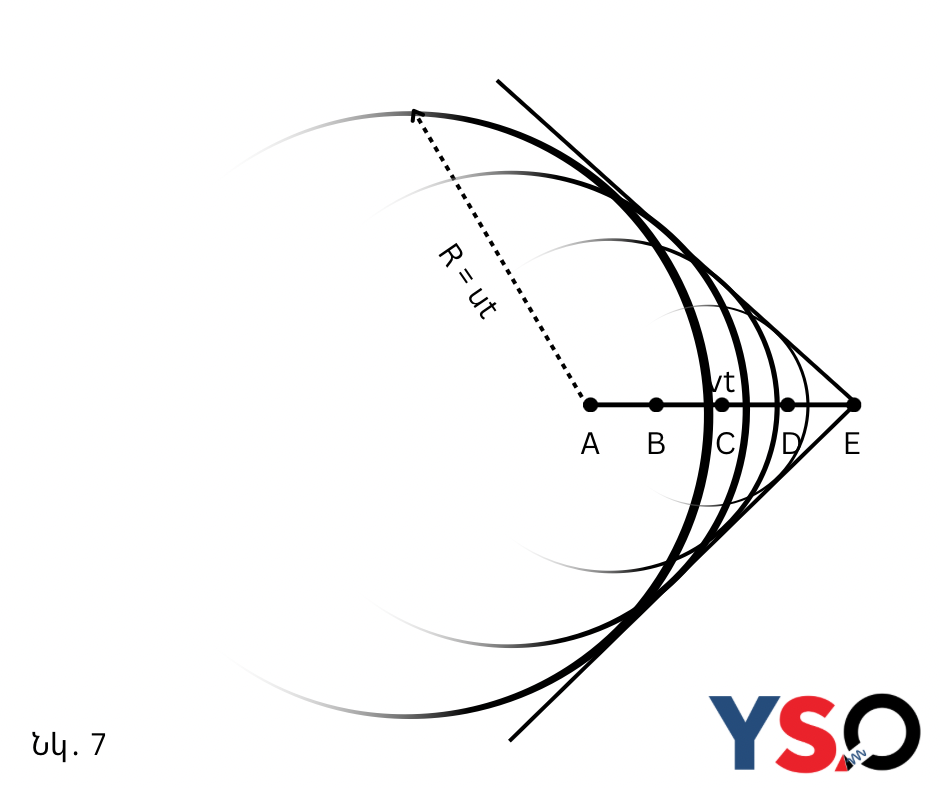
\includegraphics[width=0.6\textwidth]{images/img7.png}
  \caption{Ալիքային ճակատները, երբ $v>u$:}
  \label{fig:cone}
\end{figure}

Հենց այս երևույթի վրա հիմնվելով՝ Չերենկովն ու Վավիլովը հասկացել են, որ
միջավայրում պետք է գոյություն ունենան մասնիկներ, որոնք լույսի փուլային
արագությունից արագ են շարժվում, այլապես իրենց դիտած կապույտ ճառագայթումը
չէր դիտվի:

Ներկայումս Չերենկովյան ճառագայթումը լայն կիրառում ունի միջուկային
ֆիզիկայում՝ մասնիկների գրանցման ու օգտագործման համար:

Այս երևույթը նաև օգտագործվում է Չերենկովյան գրանցիչում, որի շնորհիվ
կարողանում են որոշել մասնիկների զանգվածները և առանձնացնել թեթև
մասնիկները, որոնց մոտ առկա է ճառագայթումը, ավելի ծանրներից, որոնց մոտ
այն չի դիտվում:

\end{document}
